\subsubsection{Scopo}
In questa sezione verranno descritti gli standard ai quali i membri del team si attengono per quanto riguarda la stesura, la \citgl{verifica} e l'approvazione dei documenti redatti. Le norme ivi indicate sono tassative per tutti i documenti formali presentati, esplicitamente riportati nella sezione "Documenti correnti".


\subsubsection{Aspettative}
Il gruppo desidera consegnare documentazione formale coerente. Per conseguire tale fine vengono seguite pedissequamente le norme relative alla documentazione ivi indicate. 

\subsubsection{Ciclo di vita della documentazione}
Ogni documento formale presentato dovrà superare con esito positivo le seguenti fasi:
    \begin{itemize}
        \item \textbf{Sviluppo}: Comprende le decisioni in merito alla strutturazione dei contenuti da comprendere nel documento e la stesura degli stessi. Il documento concluso in questo stadio è non formale. 
        
        \item \textbf{Verifica}: Quando si ritiene conclusa la stesura di un documento non formale, viene chiamato in causa il Responsabile di progetto. È sua responsabilità assegnare il documento ai Verificatori, la cui incombenza è svolgere l'attività di verifica. Quest'ultima consiste nel controllare la correttezza formale del documento. Al termine del controllo gli esiti possibili sono due:
            \begin{itemize}
                \item Esito negativo da parte dei verificatori: Nel caso in cui i Verificatori individuino degli errori o delle difformità nel documento; sarà loro dovere comunicare le proprie valutazioni al Responsabile di progetto. Quest'ultimo riassegnerà il documento ai redattori, che ripeteranno la stesura del documento o delle sue parti ritenute incorrette. Il ciclo si ripete finché i Verificatori non hanno più segnalazioni.
                \item Esito positivo da parte dei verificatori: I verificatori non individuano difformità. Il documento entra in fase di approvazione da parte del Responsabile di progetto.
            \end{itemize}
        
        \item \textbf{Approvazione}: Segue l'esito positivo della fase di verifica.
        Successivamente il documento verrà quindi passato al Project Manager, che sarà responsabile dell'approvazione o meno del documento. Gli esiti possibili sono due:
            \begin{itemize}
                \item Se il documento non viene considerato adeguato al rilascio il Responsabile di progetto comunicherà ai
                redattori le modifiche da apportare. In casi estremi, potrà imporre che la stesura del documento dovrà essere rifatta nella sua totalità.
                \item Se il documento verrà approvato lo si riterrà un documento formale, e potrà essere distribuito alle persone nominate nella lista di distribuzione.
            \end{itemize}
    \end{itemize}
A seguire è presente un diagramma rappresentante una visione schematica del ciclo di vita sopra descritto:
\begin{figure}[h!]
  \begin{center}
  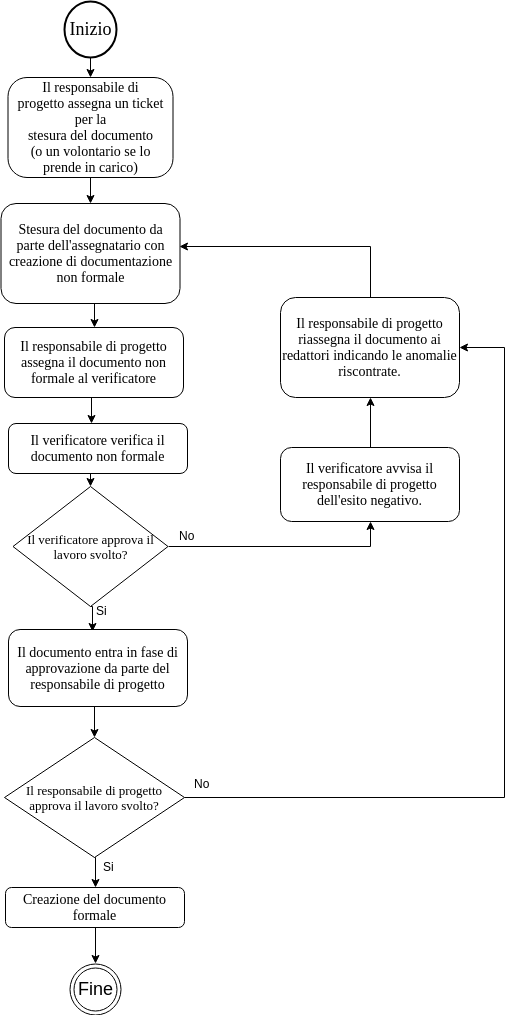
\includegraphics[scale=0.45]{immagini/Dfd.png}
  \caption{Diagramma del ciclo di vita della documentazione}
  \end{center}
\end{figure}

\newpage
\subsubsection{Separazione tra documenti interni e esterni}
I documenti formali redatti dal gruppo Cyber13 rientreranno tassativamente in una delle seguenti categorie (mutuamente esclusive):
    \begin{itemize}
        \item \textbf{Documenti interni} : Documenti ad uso esclusivo del team Cyber13, redatti in lingua Italiana.
        \item \textbf{Documenti esterni}: Documenti che verranno condivisi anche con il proponente e i committenti. Nel caso di documenti utili per il \citgl{deploy}  del software o per il loro utilizzo da parte degli utenti finali, dovranno essere redatti in lingua inglese.
    \end{itemize}

\subsubsection{Nomenclatura dei documenti}
Per quanto riguarda il nome dei documenti formali essi verranno nominati  attraverso la dicitura "NomeDocumento", senza spazi e con lettere maiuscole all'inizio di ogni parola, seguita dalla versione, nella forma: "NomeDocumento\textunderscore vX.Y.Z.estensione". \\
Per quanto riguarda i verbali (interni ed esterni) si seguirà una particolare nomenclatura, descritta nella sezione 4.1.4.3.
        
    \paragraph{Versioni di un documento} 
    ~\\
    Il numero di versione è indicato tramite il carattere ‘v’ seguito da un numero, da un punto, da un numero, da un punto e un numero: vX.Y.Z.
    Ogni volta che si inserisce una modifica nell’omonimo diario, va assegnato un nuovo numero di versione, in modo coerente con le seguenti regole:
                 \begin{itemize}
                    \item Quando verrà creato un documento avrà necessariamente il numero di versione ‘v0.0.1’.
                    \item \textbf{X}: Rappresenta il numero di pubblicazioni ufficiali del documento (quindi ogni qualvolta il documento superi con esito  positivo la fase di approvazione). Ad ogni nuova pubblicazione del documento i valori Y e Z vengono azzerati e quello di X incrementato di uno.
                     \item \textbf{Y}: Rappresenta  il  numero  di  verifiche  eseguite sul documento. L'incremento dell'indice Y implica l'azzeramento del valore dell'indice Z;
                    \item \textbf{Z}: Rappresenta il numero di modifiche effettuate al documento durante il suo sviluppo.
            \end{itemize}
    \paragraph{Formato dei file}
    ~\\
    I documenti sono redatti attraverso lo strumento Latex, pertanto ogni documento si trova nel formato .tex durante il suo sviluppo. Dopo il superamento della fase di approvazione del documento da parte del Responsabile viene il documento viene esportato in formato PDF.
         
\subsubsection{Documenti correnti}
Di seguito si presentano i documenti formali, classificati per appartenenza (interno o esterno) consegnati:
    \begin{itemize}
        \item \textbf{Analisi dei Requisiti}: Uso esterno, sigla (AdR).\\
              Documento per esporre e scomporre i requisiti del progetto contenente i
              \citgl{casi d’uso}
               relativi  al  prodotto  e  diagrammi  di  interazione  con  l’utente.   Viene scritto dagli Analisti dopo aver analizzato il capitolato e interagendo con il Proponente in riunioni esterne.
        \item \textbf{Glossario}: Uso esterno, sigla (GL). \\
              Documento per raccogliere le definizioni dei termini o concetti che saranno usati nei documenti formali per facilitarne la comprensione.
        \item \textbf{Piano di Progetto}: Uso esterno, sigla (PdP). \\
              Documento  per  l’analisi  e  la  pianificazione  della  gestione  delle  risorse  di tempo e umane.
        \item \textbf{Piano di Qualifica}: Uso esterno, sigla (PdQ). \\
              Documento per descrivere standard e obiettivi che il gruppo dovrà raggiungere per garantire la qualità di prodotto e processo.
        \item \textbf{Studio di Fattibilità}: Uso interno, sigla (SdF).\\
              Documento per indicare le riflessioni, punti di forza e caratteristiche sfavorevoli per ogni capitolato proposto sulla base dei quali il gruppo ha fatto la sua scelte.
        \item \textbf{Norme di Progetto}: Uso interno, sigla (NdP).\\
              Documento per mostrare le direttive e gli standard utilizzati all’interno del gruppo di lavoro Cyber13 per lo sviluppo del progetto.
    \end{itemize}

\subsubsection{Formattazione dei documenti}
     \paragraph {Strutturazione dei file}
     ~\\
     Ogni documento formale si deve attenere alla seguente strutturazione dei contenuti:
        \begin{itemize}
            \item \textbf{Frontespizio}: Si tratta della prima pagina dei documenti formali, conterrà le seguenti informazioni (in ordine dall'alto verso il basso):
                \begin{itemize}
                    \item Intestazione: "Università degli Studi di Padova";
                    \item Logo del gruppo: Centrato;
                    \item Titolo del documento: Centrato;
                    \item Nome del gruppo - Nome progetto: In corsivo.
                \end{itemize}
            \item \textbf{Sezione di informazione del documento}: Si trova sempre nella prima pagina del documento e contiene le seguenti informazioni:
                \begin{itemize}
                    \item Versione: Attenendosi alle norme della sezione 3.1.4.2;
                    \item Data Redazione: Seguendo il formato indicato al punto 3.1.6.2 "Formati ricorrenti";
                    \item Responsabile: Nome del responsabile che ha supervisionato il documento;
                    \item Redazione: Nomi dei redattori del documento;
                    \item Verifica: Nomi dei verificatori del documento;
                    \item Approvazione: Nome del responsabile che ha approvato il documento;
                    \item Uso: Interno o esterno;
                    \item Destinatari: A cui è indirizzato il documento;
                    \item Mail di contatto: Mail del gruppo Cyber13.
                \end{itemize}
            \item \textbf{Diario delle modifiche}: Tabella inserita nella seconda pagina del documento. Ha lo scopo di riepilogare l'elenco delle modifiche che sono state apportate al documento nel corso del processo di redazione. L'assegnamento delle versioni si attiene alle norme indicate nella sezione 3.1.4.2 "Versioni del documento".
            Il diario è una tabella ordinata in modo decrescente secondo la data della modifica e, di conseguenza, il numero di versione. Si adotta questo stile per focalizzare gli ultimi cambiamenti poiché trattati nelle prime righe della tabella.
            Ogni riga del diario dovrà contenere i seguenti elementi nell'esatto ordine in cui sono indicati:
                \begin{itemize}
                    \item Versione del documento;
                    \item Data della versione;
                    \item Descrizione delle modifiche apportate;
                    \item Autore delle modifiche apportate;
                    \item Ruolo dell'autore delle modifiche;
                \end{itemize}
            \item \textbf{Indice delle sezioni}: Gli indici hanno lo scopo di riepilogare e dare una visione macroscopica della struttura del documento. Permettono quindi di rintracciare i contenuti tramite una gerarchia. \\
            Ogni documento, esclusi i verbali, dovrà essere corredato dall'indice dei contenuti. 
            Esso sarà posizionato dopo il diario delle modifiche. Se sono presenti tabelle o immagini all'interno del documento, l’indice dei contenuti sarà seguito dalla lista delle tabelle e poi dalla lista delle figure.
            \item \textbf{Elenco delle tabelle}: Vengono indicate tutte le tabelle inserite all'interno del documento.
            \item \textbf{Elenco delle figure}: Vengono indicate tutte le figure inserite all'interno del documento.
            \item \textbf{Introduzione}: Sezione sempre presente nei documenti che ne chiarifica:
                \begin{itemize}
                    \item Scopo del documento;
                    \item Scopo del prodotto;
                    \item Riferimenti: normativi e informativi.
                \end{itemize}
            \item \textbf{Contenuto del documento}: Le restanti pagine del documento sono interamente occupate dal contenuto dello stesso. In ogni pagina, esclusa il frontespizio, devono comparire i seguenti elementi:
                \begin{itemize}
                    \item Logo del team: Dovrà comparire, nell’intestazione della pagina, il logo del gruppo Cyber13. Tale logo sarà posizionato a sinistra.
                    \item Sezione corrente: Il numero e il nome della sezione in cui ci si trova dovranno essere presenti nell'intestazione. Tali elementi saranno posizionati a destra;
                    \item Nome del documento: A piè di pagina, a sinistra, deve apparire il nome del documento completo di versione.
                    \item Numero di pagina: A piè di pagina, a destra, deve comparire il numero della pagina espresso nella seguente notazione: "Pagina x di n", dove x è la pagina corrente e n il numero di pagine totali.
                \end{itemize}
        \end{itemize}
        
     \paragraph{Norme tipografiche}
     ~\\
        \begin{itemize}
            \item \textbf{Virgolette}: Alte singole ’ ’ per singolo carattere,  alte doppie ” ” per racchiudere stringhe mentre parentesi angolari <<  >> per racchiudere citazioni.
            \item \textbf{Parentesi}: Tonde  per  descrivere  esempi  e  fornire  sinonimi  o  precisazioni, quadre per rappresentare uno \citgl{standard} \citgl{ISO}, uno stato relativo a un
            \citgl{ticket}
             o un riferimento ad un codice definito all'interno del documento stesso.
            \item \textbf{Punteggiatura}: Ogni  segno  di  punteggiatura  deve  essere  seguito  da  uno spazio e non avere spazi precedenti al segno stesso;
            \item \textbf{Stile del testo}:
                \begin{itemize}
                    \item Corsivo: Per dare enfasi ad una parola, un concetto o per indicare il nome di un
                    termini di glossario e nomi di  documenti.
                    \item Grassetto: Per i titoli, sottotitoli ed elementi di elenchi e liste di definizione di primo livello.
                    \item Azzurro: Per indicare dei collegamenti ipertestuali.
                \end{itemize}
            \item \textbf{Elenchi}: La prima parola di ogni punto appartenete a un elenco inizierà con la lettera maiuscola. In caso di elenchi di definizioni, al termine da definire seguiranno i ’due punti’ (:)  successivamente vi sarà la sua descrizione. Al termine della descrizione dell'elemento si inserirà il carattere ’punto e virgola’ (;) nel caso di definizione semplice, mentre il carattere 'punto' (.) al termine di una definizione complessa (più di un periodo).
            Per l’ultimo elemento della lista si userà sempre il carattere ’punto’ (.);
            \item \textbf{Formati ricorrenti}:
                \begin{itemize}
                    \item Date: Scritte con lo standard YYYY-MM-DD dove YYYY indica l’anno, MM il mese e DD il giorno;
                    \item Orari: Scritti nel formato 24h.
                \end{itemize}
            \item \textbf{Componenti grafiche}:
                \begin{itemize}
                    \item Immagini: I formati ammessi sono PNG o JPG;
                    \item Tabelle: Devono rispettare lo stile del \citgl{template} \citgl{Latex} realizzato.
                \end{itemize}
        \end{itemize}


\subsubsection{Ambiente}
La stesura dei documenti deve essere effettuata utilizzando il \citgl{linguaggio di markup}
\citgl{LaTeX} e l’ambiente \citgl{Overleaf} con dizionario italiano ed inglese installati.

